\chapter{Présentation du sujet}
Mon sujet s'inscrit dans un projet developpé en interne, le projet SisellBox. Ainsi,
je vais présenter dans un premier temps le projet, puis dans un second temps,
expliquer où je m'inscrit dans le projet et ce que j'y ai contribué.



\section{Le projet SisellBox}
\label{sisselbox}

\begin{figure}[!h]
  \centering
  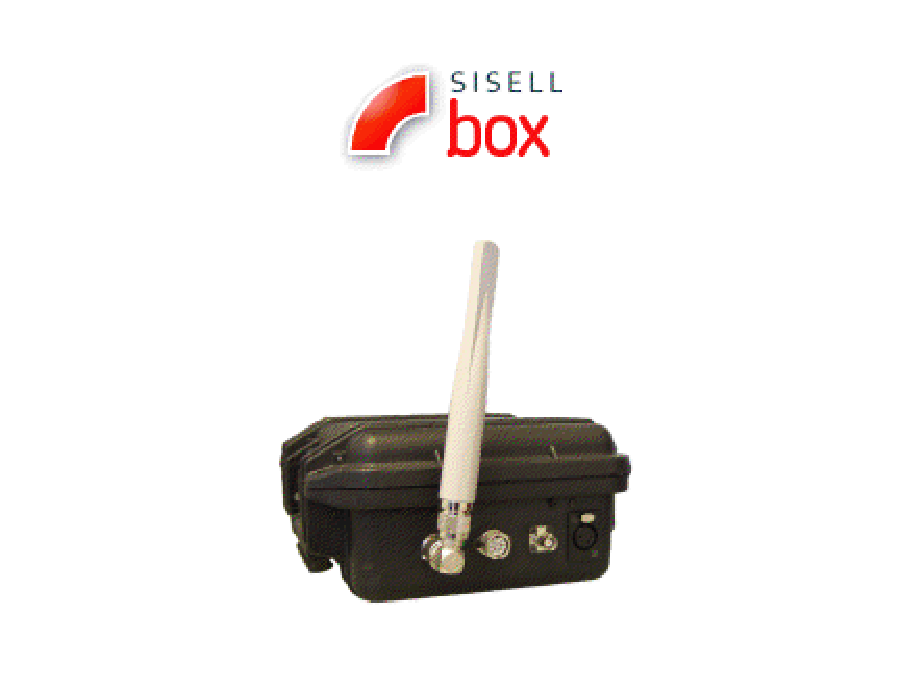
\includegraphics[scale=0.7]{figures/sbox}
  \caption{image de la SisellBox}
\end{figure}
\newpage
La SisellBox est un enregistreur développé par Open Wide permettant de déployer une solution complète de vidéo surveillance rapidement.
Ce système peut être utilisé dans des contextes de mission très différents : surveillance longue durée, protection de sites sensibles, capture d'images en hautes qualité, ainsi que surveillance ponctuelle.
Fonctionnant sur batterie et créant un réseau wifi maillé de façon autonome, elle ne nécessite que peu d'intervention humaine pour l'utilisation. Il suffit de brancher la batterie, brancher les caméras . L'utilisation d'algorithmes performants lui permet de détecter et d'analyser tout événement (intrusion, stationnarité, mouvement de foule) sur la base de critères précis et configurables. Le projet SisellBox se découpe en partie, deux partie, d'une part le "streamer", prenant en entrée une source vidéo "live"(par exemple une caméra de sécurité) et fournit un flux de composé de vidéo et de métadonnées. La deuxième partie, le "recorder" récupère les flux vidéo et de méta-données générées par le streamer. Les méta-données sont enregistrées en base de données ainsi que diverses informations (localisation des enregistrements vidéo entre autres)

\subsection{SisellBox Streamer}
La partie streamer de SisellBox gère la capture vidéo, l'analyse de l'image et son émission sur un réseau.

\begin{figure}[!h]
  \centering
  \includegraphics[scale=0.7]{figures/sisell_box}
  \caption{Cas d'utilisation du streamer}
\end{figure}

Afin de faciliter l'inter-opérabilité de cette application, il faut se baser sur des protocoles de communications standards. La norme ONVIF, qui a pour objectif d'uniformiser les services de vidéosurveillance , préconise d'utiliser le protocole RTSP pour les émissions de flux vidéo. Le protocole RTSP (Real Time Streaming Protocol) est un protocole destiné aux systèmes de streaming multimédia. Il permet de contrôler le média à distance (jouer, mettre en pause, enregistrer, fin de session etc. ). Cela permet donc de ne pas se soucier de l’implémentation de ces fonctionnalités côté serveur et permettre le contrôle du flux via un lecteur standard type VLC sans développement supplémentaire. Le RTSP ne gère par contre pas la partie transport des données. Celles-ci sont donc émises via le protocole de transport RTP (Real-time Transport Protocol). Ainsi furent les choix technologiques pris avant mon arrivé sur le projet. Or, il s'est avéré que la norme ONVIF était trop compliquée à implémenter avec Gstreamer dû à des limitations technologiques. Il a été choisi d'encapsuler le flux de données au travers de MPEG-TS puis de le transmettre via RTP.\\
L’image capturée par le streamer peut ensuite être analysée par une ou plusieurs brique(s) d’analyse. Une brique d'analyse est un élément interchangeable effectuant un traitement particulier sur l'image afin d'en extraire des informations (détection de visages, reconnaissance de formes, mouvements, etc..). Actuellement, seuls quelques algorithmes d'analyse (tel que la détection de visage) ont été implémentés pour la nouvelle architecture.\\
Les informations extraites par la brique d'analyse sont mises sous la forme de métadonnées. Chaque trame vidéo se voit donc associée à une trame de métadonnée. Celle-ci peut être vide si aucune information n'a été extraite par l'algorithme d'analyse vidéo, mais, est ,néanmoins,  présente.
Le flux vidéo peut être encodé avec les formats H.264 et MJPEG, afin de les transmettre sur le réseau. Le streamer doit aussi gérer des sources non-live (fichiers vidéos) de différents formats (*.mkv, *.ts, *.avi).\\
Du côté de l'implémentation, les briques algorithmiques de traitement d'image sont développées en C++ et en Vala. Le reste est développé en Python et en utilisant les bindings Python pour GStreamer afin d'utiliser le framework et ses plugins développés en C.


\subsection{SisellBox Recorder}
Le recorder récupère les flux vidéo et de méta-données généré par le streamer. Les méta-données sont enregistrées en base de données ainsi que diverses informations (localisation des enregistrements vidéo etc.). La vidéo est multiplexé avec les méta-données (en utilisant la piste de sous-titres) puis enregistrée sur le disque. Le recorder peut également récupérer des images (format .jpeg) d'une zone de la vidéo récupérée (par exemple un visage détecté en amont) via un élément « Snapshoter ».

\begin{figure}[!h]
  \centering
  \includegraphics[scale=0.5]{figures/sisell_box_recorder}
  \caption{Cas d'utilisation du recorder}
\end{figure}

Le recorder est capable de :
\begin{itemize}
\item Recevoir des flux vidéo et de méta-données et compatible avec au minimum :
    \begin{itemize}[label=$\bullet$]
      \item  protocoles réseau : RTSP/RTP
      \item  codecs : MJPEG et H.264
    \end{itemize}
\item Enregistrer les vidéos sur disque dans un format permettant de les relire ainsi que les méta-données associés, dans notre cas, nous utilisons un conteneur MPEG-TS (fichier *.ts) avec les codecs H.264 et MJPEG pour la vidéo et du binaire formatés pour les méta-données
\item Stocker les métadonnées en base de donnée
\item Effectué des enregistrements sur des événements. Les événements pouvant être de type :
  \begin{itemize}[label=$\bullet$]
      \item Présence de méta-données
      \item  événement de type particulier (présence de personne, … )\\
  \end{itemize}
\end{itemize}

Pour la base de données, nous utilisons PostgreSQL et Postgis (extension de PostgreSQL pour la manipulation d'informations géographiques) sur une machine Debian distante. Pour la phase de développement, cette machine est virtualisée via une VM VirtualBox.
Les lectures/écritures dans la base de donnée depuis le recorder se font grâce un mapping objet-relationnel (ORM) permettant de manipuler une base de données relationnelles de la même manière qu'une base de données orienté objet. Pour cela nous utilisons l'outil libre SQLAlchemy.


\chapter{Les problématiques posées}
Ainsi, après avoir explicité le contexte du projet, il est temps que je décrive les différentes problématique qui m'ont été posées durant ce stage. Dans un premier temps, le projet repose sur le framework multimédia Gstreamer\footnote{cet technologie est décrite plus en détaille ici \ref{gstreamer}}, n'ayant jamais rencontré cet technologie auparavant, il m'a fallu un temps  	d'auto-formation afin d'acquerir les bases pour pouvoir commencer le développement de plugins simples. Ensuite, il m'as fallut étudier les plugins qui implémente le multiplexage et démultiplexage des données dans les fichiers MPEG-TS afin de pourvoir patcher le code.